\section{Materials and Methods}
\label{sec:methods}

This section describes the research framework: dataset, preprocessing, classification model, training configuration, the five XAI methods and the proposed consistency metric, the evaluation protocol, and implementation details. Fig.~\ref{fig:1} summarises the pipeline. A site-unlabelled ultrasound dataset release is used (Section~\ref{sec:methods}.1), a ResNet-50 \cite{ref27} classifier is trained end-to-end on it, and an XAI module then applies all five methods of Section~\ref{sec:methods}.3 to the same trained model. Quantitative evaluation follows, through grounded failure-case analysis and cross-replicate explanation consistency, feeding into the validation roadmap of Section~\ref{sec:future-research}.

\begin{figure}[p]
\centering
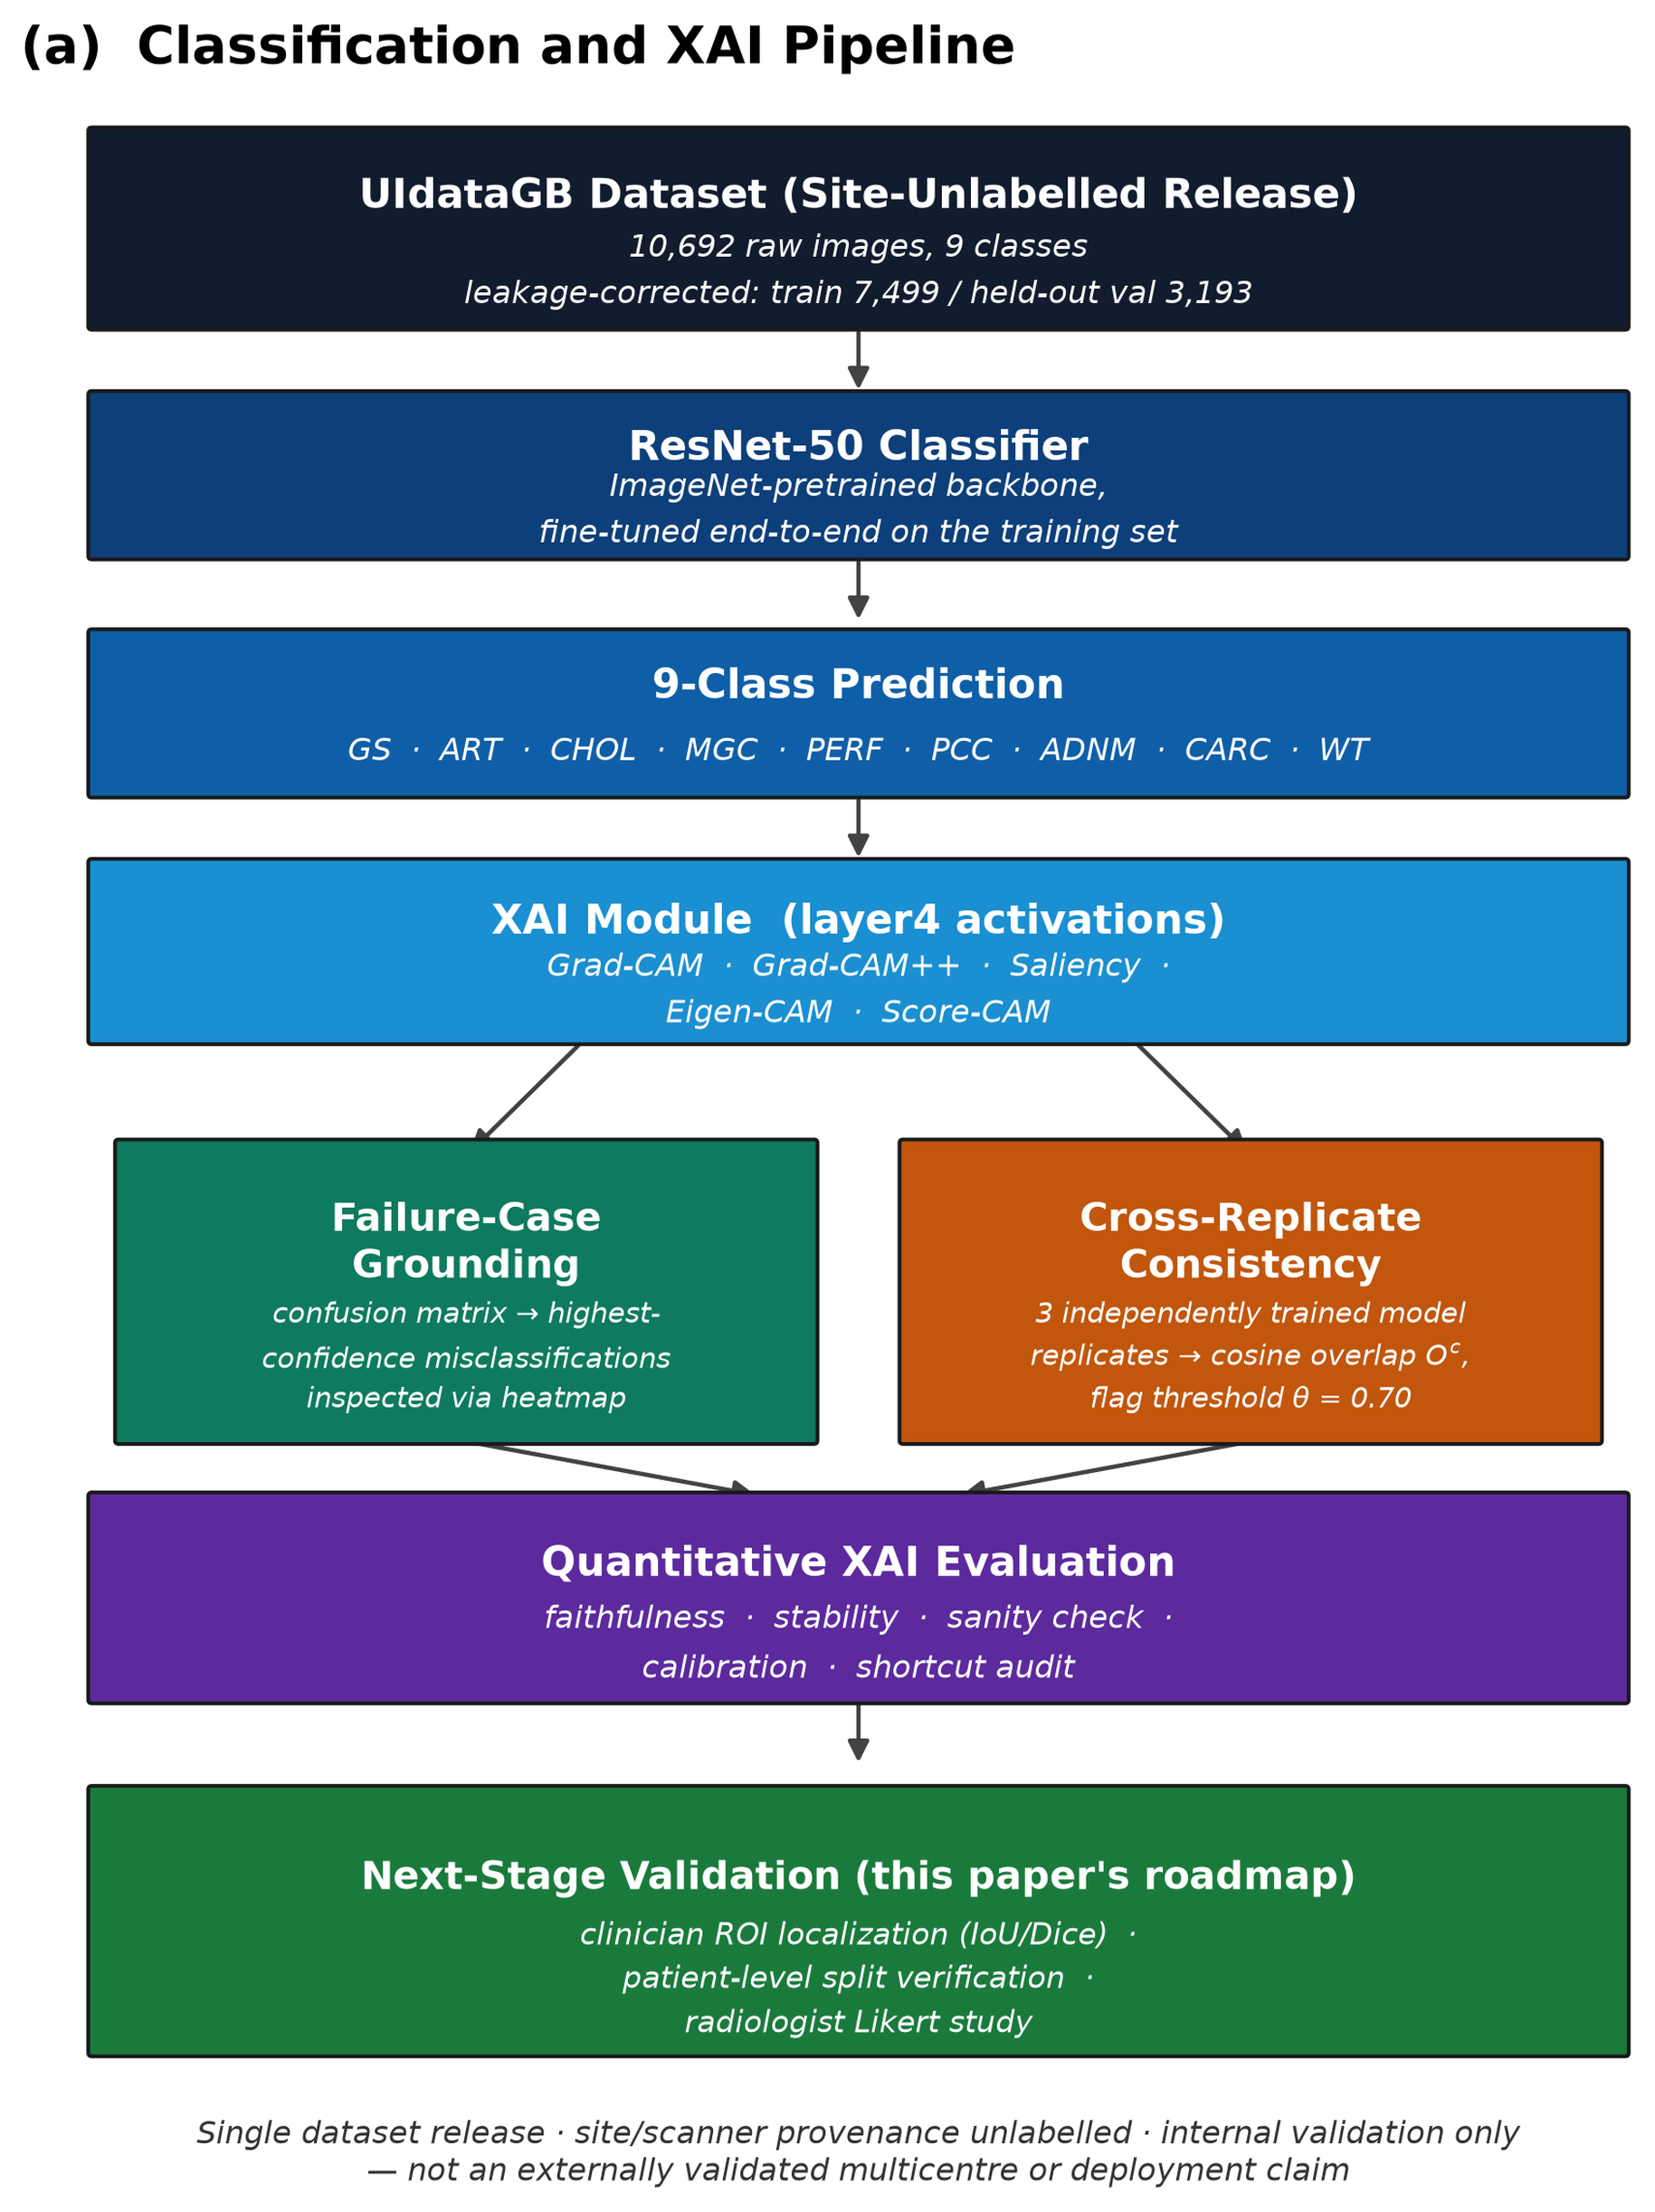
\includegraphics[width=0.92\linewidth]{figures/xai_pipeline_diagram_final}

\vspace{10pt}

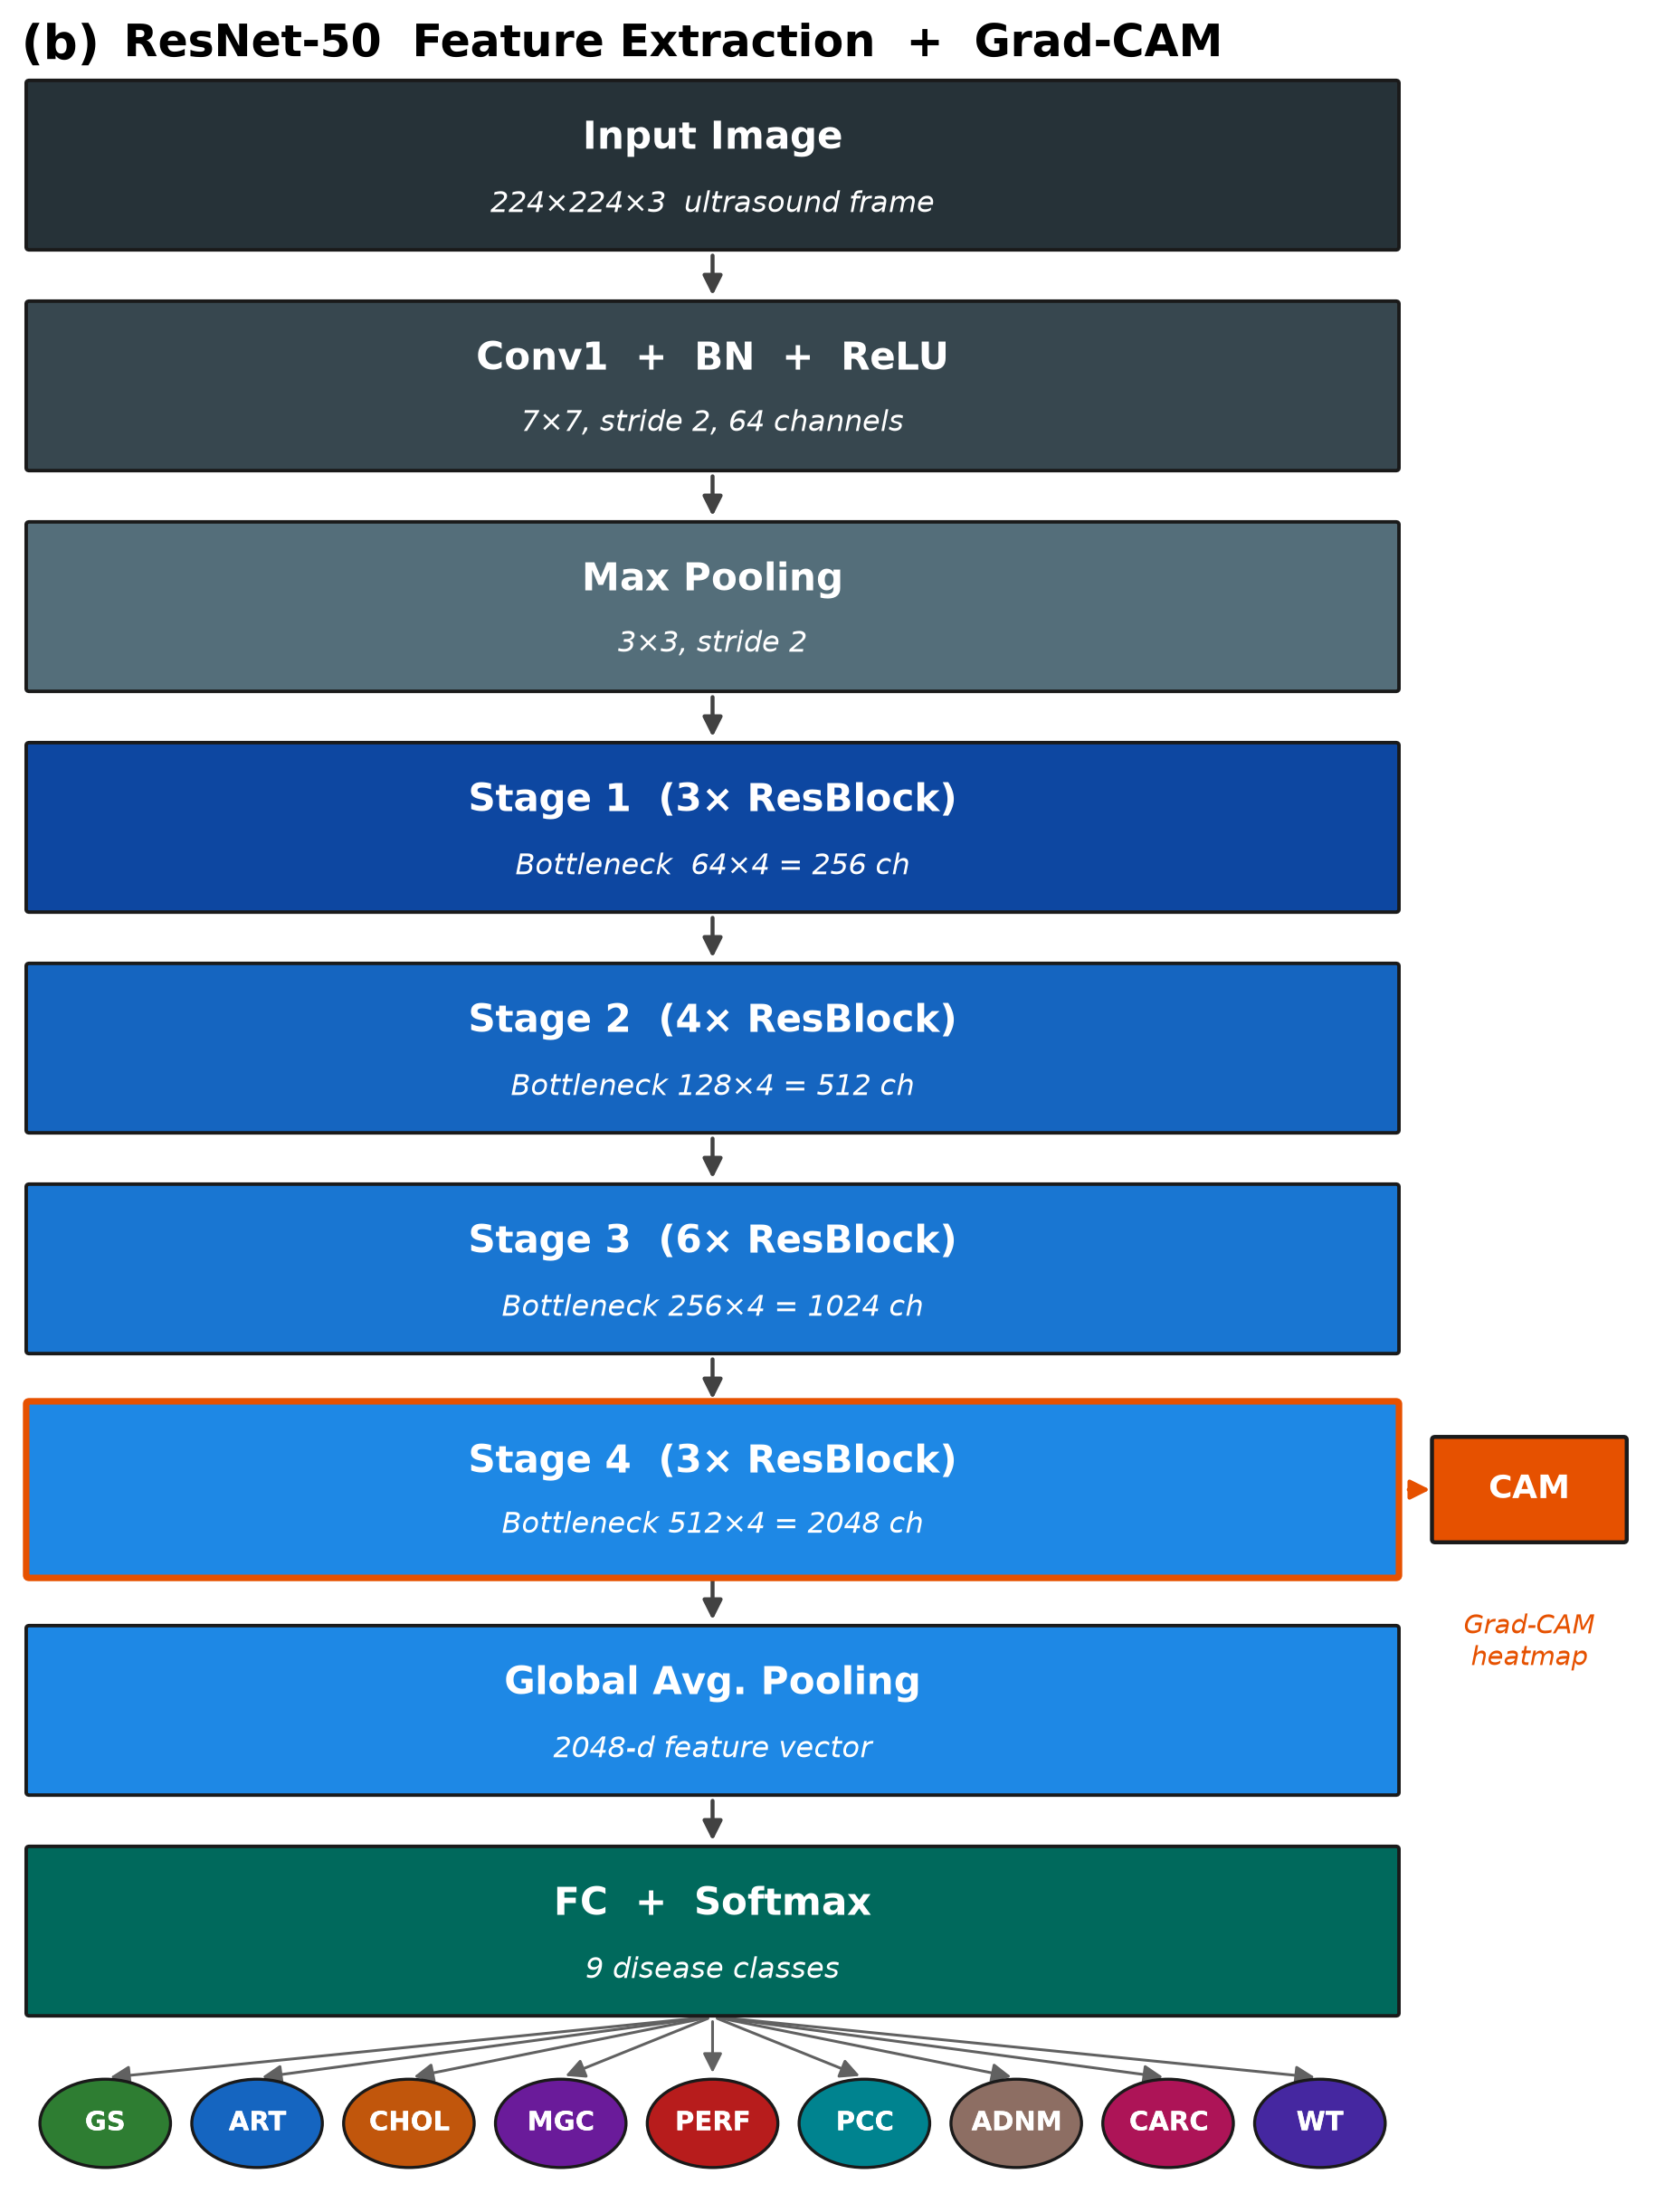
\includegraphics[width=0.92\linewidth]{figures/resnet_backbone_final}

\vspace{8pt}
\caption{(a)~End-to-end classification and XAI pipeline used in this paper, run on a site-unlabelled public dataset release. (b)~ResNet-50 backbone: all four CAM-family methods tap the Stage~4 (\texttt{layer4}) activations, the highest-level convolutional features before global average pooling. Both panels are rendered at identical scale for direct visual comparison.}
\label{fig:1}
\end{figure}

\subsection{Dataset description}

This study uses the publicly available UIdataGB dataset \cite{ref17}, a multi-class gallbladder ultrasound image collection spanning nine disease classes: Gallstones (GS), Abdomen \& Retroperitoneum (ART), Cholecystitis (CHOL), Membranous/Gangrenous Cholecystitis (MGC), Perforation (PERF), Polyps \& Cholesterol Crystals (PCC), Adenomyomatosis (ADNM), Carcinoma (CARC), and Wall Thickening (various causes, WT). Part of the collection was assembled from video-cine sequences, which can produce near-identical consecutive frames, so the released train/validation split was de-duplicated at the image-cluster level using perceptual hashing (64-bit pHash, Hamming distance~$\le 8$ treated as a near-duplicate) before any classification or XAI result was computed. That way, reported performance reflects genuine generalisation rather than memorised near-duplicates.

\textbf{Final dataset statistics.} The de-duplicated split comprises 7,499 training and 3,193 validation images (Table~\ref{tbl:1}, Fig.~\ref{fig:2}). Carcinoma is the largest class (1,590 images total) and Wall Thickening the smallest (990), but as Section~\ref{sec:results}.1 shows, the weakest-performing classes (Perforation, Gallstones) are not simply the smallest ones: class size alone does not explain the per-class performance profile.

\begin{table}[!ht]
\centering
\caption{UIdataGB Dataset Statistics: Class Distribution across Train / Validation Splits.}
\label{tbl:1}
\begin{tabular}{lccc}
\toprule
Class & Train & Validation & Total \\
\midrule
Gallstones (GS) & 927 & 399 & 1326 \\
Abdomen \& Retroperitoneum (ART) & 807 & 363 & 1170 \\
Cholecystitis (CHOL) & 795 & 351 & 1146 \\
Membranous/Gangrenous Cholecystitis (MGC) & 868 & 356 & 1224 \\
Perforation (PERF) & 742 & 320 & 1062 \\
Polyps \& Cholesterol Crystals (PCC) & 734 & 286 & 1020 \\
Adenomyomatosis (ADNM) & 813 & 351 & 1164 \\
Carcinoma (CARC) & 1120 & 470 & 1590 \\
Wall Thickening, various causes (WT) & 693 & 297 & 990 \\
\midrule
\textbf{Total} & \textbf{7499} & \textbf{3193} & \textbf{10692} \\
\bottomrule
\end{tabular}
\end{table}

\begin{figure*}[!ht]
\centering
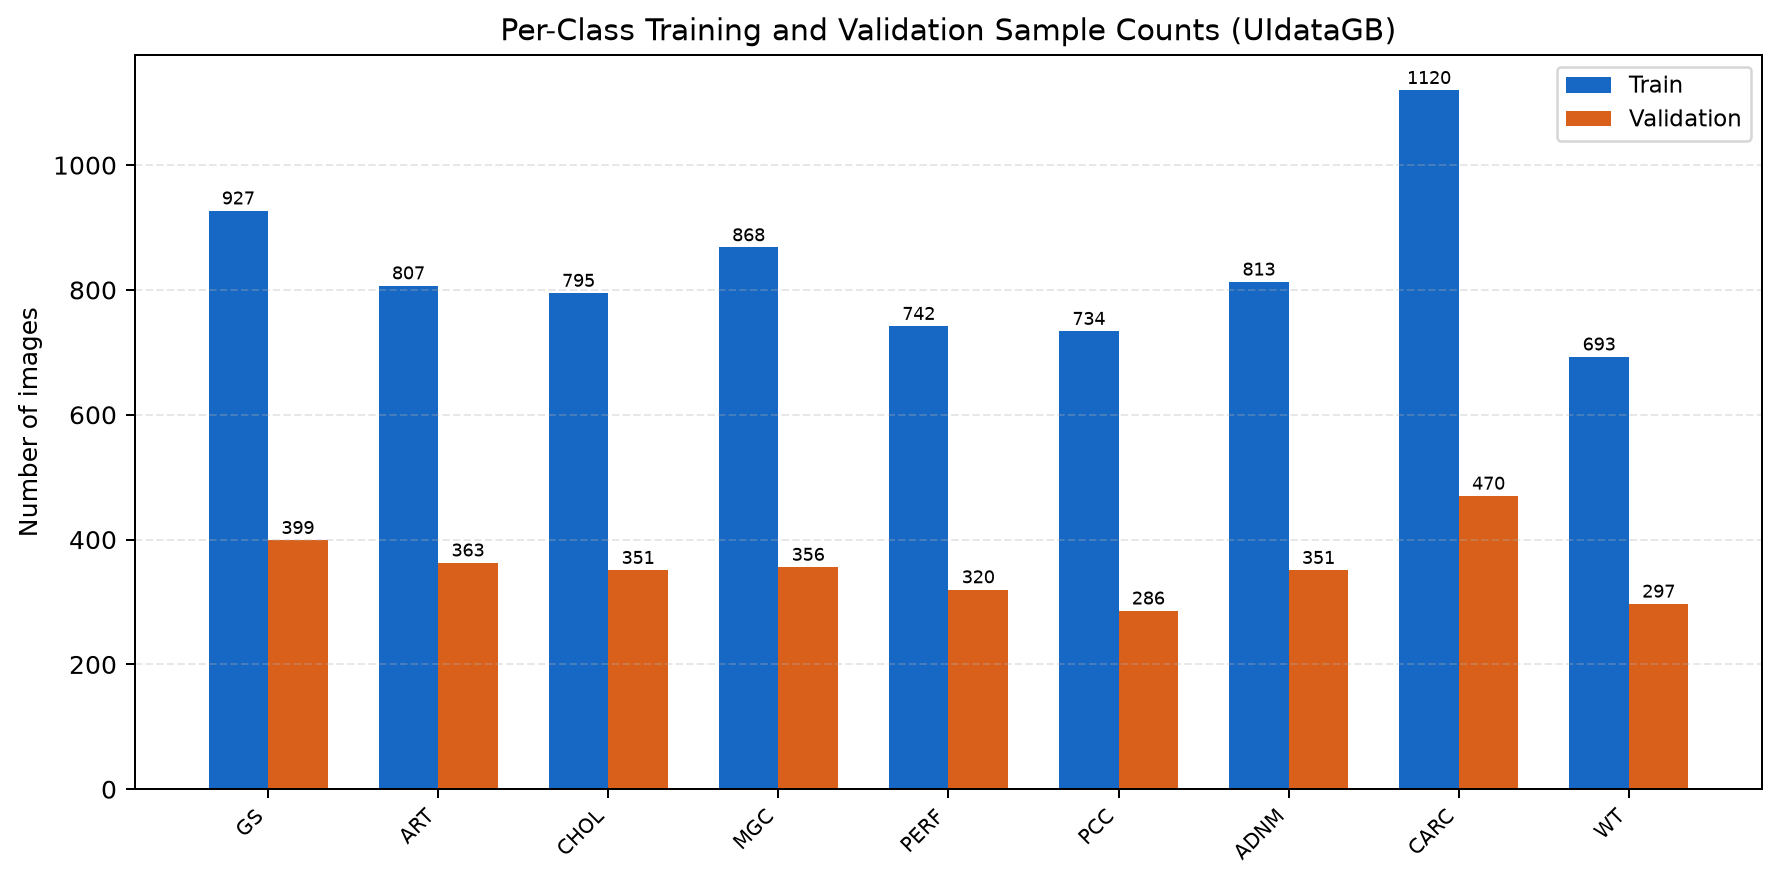
\includegraphics[width=0.75\textwidth]{figures/dataset_statistics.png}
\caption{Per-class training and validation sample counts (Table~\ref{tbl:1}). Carcinoma is the largest class (1,590 images); Wall Thickening is the smallest (990).}
\label{fig:2}
\end{figure*}

\subsection{Classification model and training configuration}

Images are resized to $224\times224$ and normalized using ImageNet statistics. Standard augmentations (random horizontal flip, $\pm15^\circ$ rotation, brightness/contrast jitter) \cite{ref43} are applied during training only, not at validation time, and standard cross-entropy is used (Table~\ref{tbl:2}) rather than a class-imbalance-aware loss such as focal loss \cite{ref44}. A weighted or focal-loss ablation is a natural next step given the class imbalance in Table~\ref{tbl:1}, and is left for future work.

ResNet-50 \cite{ref27} pretrained on ImageNet \cite{ref30} is adopted as the feature extractor, with the final fully-connected layer replaced by a nine-class classification head: Dropout($p=0.4$)~$\rightarrow$~Dense(256, ReLU)~$\rightarrow$~Dropout($p=0.3$)~$\rightarrow$~Dense(9). The head outputs raw logits over the nine classes of Table~\ref{tbl:1}. Training uses \texttt{nn.CrossEntropyLoss} (Table~\ref{tbl:2}), which expects raw logits and applies log-softmax internally, while softmax is applied only at inference time to obtain the reported probabilities and confidence values (Section~\ref{sec:results}.4); no softmax layer is part of the trained model itself. ResNet-50's residual structure and deep feature hierarchy make it well suited to CAM-family explanation methods, since the \texttt{layer4} output encodes rich semantic features prior to global average pooling. It was chosen over deeper or more parameter-efficient alternatives such as DenseNet-121 \cite{ref28} or EfficientNet \cite{ref29} mainly for comparability with prior gallbladder-ultrasound baselines \cite{ref7}, which are themselves ResNet-based; comparing backbones is not this paper's focus.

\begin{table}[!ht]
\centering
\caption{Hyperparameter and Training Configuration.}
\label{tbl:2}
\begin{tabular}{ll}
\toprule
Hyperparameter & Value \\
\midrule
Backbone & ResNet-50 (ImageNet) \\
Optimizer & Adam, $\beta_1{=}0.9$ \\
Learning rate & $1\times10^{-4}$ \\
Weight decay & $1\times10^{-4}$ \\
Loss function & Cross-entropy \\
Batch size & 32 \\
Training epochs & 10 \\
Replicate models $R$ & 3 \\
Train / Val split & 70\% / 30\% (cluster-level, Section~\ref{sec:methods}.1) \\
Framework & PyTorch~2.x, torchvision~0.15 \\
Model parameters & 24.03M (all trainable) \\
Checkpoint size & 96~MB (fp32) \\
Inference latency & 187~ms/image (CPU, 4 threads); ${\sim}44$~ms (GTX~1050) \\
\bottomrule
\end{tabular}

\vspace{2pt}
\raggedright\footnotesize Latency is architecture-bound, not class-count-bound (a 9-way vs. 5-way softmax head differs by a negligible 2,048$\times$4 parameters), so the measured value from the identical ResNet-50/GTX~1050 setup is unchanged.
\end{table}

\subsection{Explainability methods and consistency metric}

Five complementary visual-explanation methods are applied to the trained ResNet-50 model. Four of them target the final convolutional layer (\texttt{layer4}), which encodes the highest-level semantic features before global average pooling, while the fifth (Saliency) operates directly in pixel space. Let $A^k \in \mathbb{R}^{H \times W}$ denote the $k$-th feature map of the target layer, and let $y^c$ be the class score for class $c$ before softmax.

\textbf{1)~Grad-CAM:} Grad-CAM \cite{ref11} computes a class-discriminative localization map by weighting each feature map $A^k$ with the global-average-pooled gradient of $y^c$ with respect to that map:
\begin{equation}
\alpha_k^c = \frac{1}{Z}\sum_i\sum_j \frac{\partial y^c}{\partial A^k_{ij}},
\end{equation}
\begin{equation}
L^c_{\text{GradCAM}} = \mathrm{ReLU}\!\left(\sum_k \alpha_k^c A^k\right).
\end{equation}
The ReLU discards negative activations, retaining only positive evidence. The resulting heatmap is upsampled to $224\times224$ and overlaid on the input image.

\textbf{2)~Grad-CAM++:} Grad-CAM++ \cite{ref12} extends Grad-CAM using a pixel-wise weighted average of second-order partial derivatives, giving more weight to pixels where the gradient is strong and locally peaked, producing sharper localization for small or multiple lesions:
\begin{equation}
\alpha_k^{c,++} = \sum_{i,j} \frac{(\partial^2 y^c / \partial (A^k_{ij})^2)}{2(\partial^2 y^c / \partial (A^k_{ij})^2) + \sum_{a,b} A^k_{ab}\,(\partial^3 y^c / \partial (A^k_{ij})^3)},
\end{equation}
\begin{equation}
L^c_{\text{GradCAM++}} = \mathrm{ReLU}\!\left(\sum_k \alpha_k^{c,++} A^k\right).
\end{equation}
\textit{Equation--implementation cross-check:} this presentation follows the pixel-wise weighting structure of Chattopadhay et~al.~\cite{ref12}; before this manuscript is finalised, both the equation above and the \texttt{gradcam.py} implementation should be checked line-by-line against the original paper's Eq.~(4)--(19) to confirm no compression or transcription error, since the two must match exactly for the reported results to be reproducible from the stated formula.

\textbf{3)~Saliency Maps:} Gradient saliency \cite{ref33} computes the gradient of the class score $y^c$ with respect to the input image pixels $\mathbf{x} \in \mathbb{R}^{3 \times H \times W}$:
\begin{equation}
S^c = \left|\frac{\partial y^c}{\partial \mathbf{x}}\right|.
\end{equation}
This highlights pixel-level evidence in input space rather than feature-map space. It is noisier than Grad-CAM, but requires no target-layer choice and captures fine-grained texture cues, and it still requires differentiable, white-box access to the model's gradients: architecture-agnostic in that it needs no CAM-style layer tap, but not model-agnostic in the stricter input/output-only sense of methods such as LIME or SHAP. For visualisation, the maximum over colour channels is taken and Gaussian smoothing applied ($\sigma=1$).

\textbf{4)~Eigen-CAM:} Eigen-CAM \cite{ref34} is class-agnostic: it reshapes the target-layer activation tensor $A \in \mathbb{R}^{K \times HW}$ and computes its dominant direction of variation via singular value decomposition, $A = U\Sigma V^{\!\top}$, projecting onto the first principal component to obtain an $HW$-dimensional saliency map reshaped back to $H \times W$. Because Eigen-CAM does not condition on class $c$, it highlights the single dominant activation pattern in the layer regardless of the predicted class. This makes it useful as a lightweight, gradient-free baseline, but with weaker class-discriminative power than the methods above. \textit{Equation--implementation cross-check:} the exact projection expression and matrix orientation above should be verified against Muhammad and Yeasin's original formulation~\cite{ref34} and the \texttt{gradcam.py} implementation before this manuscript is finalised, to confirm the dimensions of $A$, $U$, $\Sigma$, $V$ are stated consistently throughout.

\textbf{5)~Score-CAM:} Score-CAM \cite{ref35} is gradient-free: each channel's importance weight is obtained by masking the input image with that channel's (upsampled, normalised) activation map and measuring the resulting change in the model's own softmax score for class $c$,
\begin{equation}
\alpha_k^{c,\text{score}} = f^c\big(\mathbf{x}\odot \text{Up}(A^k)\big) - f^c(\mathbf{x}_b),
\end{equation}
\begin{equation}
L^c_{\text{ScoreCAM}} = \mathrm{ReLU}\!\left(\sum_k \alpha_k^{c,\text{score}} A^k\right),
\end{equation}
where $f^c(\cdot)$ is the softmax score for class $c$ and $\mathbf{x}_b$ a baseline (blank) input. Because the weighting is derived directly from the model's forward-pass behaviour rather than from gradients, Score-CAM avoids gradient saturation and noise, at the cost of one forward pass per channel (computed here on GPU).

After training, all five methods above are applied to the primary model $M_0$ and to each of the three replicate models $\{M_1,M_2,M_3\}$ (Section~\ref{sec:methods}.3), using the same input images, which allows consistency scores to be computed for every class and method. Algorithm~\ref{alg:1} formalises the pipeline.

\begin{algorithm}[tb]
\caption{XAI Pipeline with Consistency Scoring}
\label{alg:1}
\begin{algorithmic}[1]
\Require primary model $M_0$, replicate models $\{M_r\}_{r=1}^{3}$, test image $\mathbf{x}$, class set $\mathcal{C} = \{$GS, ART, CHOL, MGC, PERF, PCC, ADNM, CARC, WT$\}$, target conv layer $\ell^*$, threshold $\theta$
\Ensure heatmaps per method and model, consistency scores $O_r^c$
\For{method $m \in \{$GradCAM, GradCAM++, Saliency, EigenCAM, ScoreCAM$\}$}
  \For{$c \in \mathcal{C}$}
    \State $L^c_{\text{primary}} \leftarrow \text{XAI}_m(\mathbf{x};\,M_0,\,c,\,\ell^*)$
    \State Upsample $L^c_{\text{primary}}$ to $224{\times}224$; overlay on $\mathbf{x}$
    \For{each replicate $r \in \{1,2,3\}$}
      \State $L^c_r \leftarrow \text{XAI}_m(\mathbf{x};\,M_r,\,c,\,\ell^*)$
      \State $O_r^c \leftarrow \dfrac{\langle L^c_{\text{primary}},\,L^c_r\rangle}{\|L^c_{\text{primary}}\|\cdot\|L^c_r\|}$
      \If{$O_r^c < \theta$}
        \State flag as explanation-divergent
      \EndIf
    \EndFor
  \EndFor
\EndFor
\State \Return all heatmaps, $\{O_r^c\}$ per method
\end{algorithmic}
\end{algorithm}

A heatmap that looks anatomically plausible for one trained model is not, by itself, evidence that the explanation reflects a stable property of the learned decision boundary rather than an artifact of that specific training run. To test this, a cosine-consistency score is defined between the primary model's heatmap and each of $R{=}3$ independently trained replicate models' heatmaps, for the same class and image:
\begin{equation}
O_r^c = \frac{\langle L^c_{\text{primary}},\, L^c_r \rangle}{\|L^c_{\text{primary}}\| \cdot \|L^c_r\|},\qquad r=1,\dots,R,
\end{equation}
where both heatmaps are flattened and normalised to $[0,1]$ before computing cosine similarity. Because $O_r^c \in [0,1]$, a value near 1 means the two independently trained models produce essentially the same explanation for class $c$, while a value near 0 means the explanation is training-run dependent rather than a robust model property. A threshold of $\theta = 0.70$ flags class/replicate pairs whose explanations diverge substantially, though this threshold is operational and exploratory rather than an established, validated cut-off for explanation agreement: no clinical or XAI-specific validation of a universal 0.70 threshold is known to the authors, and it is the continuous similarity score, not the binary flag, that is treated as the primary quantity throughout Section~\ref{sec:results}.3.

All classification results in Section~\ref{sec:results}.1 come from one primary model, $M_0$, trained on the full 7,499-image corrected training set with no resampling. To compute $O^c$, three additional replicate models $\{M_1,M_2,M_3\}$ are trained on three disjoint subsets of that same corrected training set (2,749, 2,089, and 2,661 images respectively); these are training-resampling replicates, not independent clinical sites. Each subset has a different per-class composition by construction, so $O^c$ jointly probes robustness to both re-initialisation and moderate class-distribution shift. Running all five XAI methods on four models over the full 3,193-image validation set is computationally expensive, so $O^c$ is instead computed on a stratified subset of 8 images per class (72 total); the faithfulness, stability, and sanity-check batteries of Section~\ref{sec:results}.4 use larger stratified samples of 144, 216, and 108 images respectively. This remains a reproducibility check on the explanation, not a multicentre or domain-shift experiment. Genuine cross-site validation instead requires images with known, traceable hospital or scanner identity, which this dataset's public release does not provide (Section~\ref{sec:limitations}, Section~\ref{sec:future-research}).

\subsection{Evaluation protocol}

\textbf{1)~Classification Metrics:} Classification performance is reported as Accuracy, Macro-F1, AUC-ROC (one-vs-rest) \cite{ref45}, and per-class Sensitivity and Specificity. Given the class imbalance in Table~\ref{tbl:1}, ROC-AUC should be read alongside per-class sensitivity rather than in isolation, since precision-recall curves can be more informative for rarer classes under imbalance \cite{ref46}; it is retained mainly for continuity with prior gallbladder-ultrasound baselines \cite{ref7}, \cite{ref19}, \cite{ref20}, \cite{ref21}. Per-class F1 and AUC (Table~\ref{tbl:4}) provide the classification context within which XAI results should be interpreted, and classes with low F1 (Perforation, Gallstones) are the primary targets for XAI investigation.

\textbf{2)~XAI Evaluation Metrics:} XAI quality is evaluated along seven dimensions: (1)~\textbf{anatomical plausibility}, a visual check of whether heatmaps concentrate on gallbladder wall, lumen, and adjacent tissue rather than artefacts (Section~\ref{sec:results}.3); (2)~\textbf{cross-method comparison}, both qualitative and quantitative, across all five methods (Section~\ref{sec:results}.3); (3)~\textbf{cross-replicate consistency}, the $O^c$ score of Section~\ref{sec:methods}.3, with $\theta=0.70$ as the divergence threshold (Section~\ref{sec:results}.3); (4)~\textbf{faithfulness}, via deletion/insertion curves against a random control (Section~\ref{sec:results}.4); (5)~\textbf{stability}, the explanation's agreement under clinically invariant transforms (Section~\ref{sec:results}.4); (6)~a \textbf{model-randomization sanity check} (Section~\ref{sec:results}.4); and (7)~a \textbf{shortcut-learning audit} (Section~\ref{sec:results}.4). SSIM, Pearson correlation, and top-decile IoU quantify agreement in (5), and deletion/insertion AUC quantifies (4). The one dimension this paper does \textit{not} establish is localization of the explanation against clinician-annotated regions of interest, which needs expert annotation and is scoped as the immediate next step (Section~\ref{sec:future-research}).

A classifier can be accurate yet miscalibrated, since its softmax confidence need not match its true correctness rate \cite{ref42}. A single scalar temperature $T>0$ is therefore fit post-hoc on a held-out calibration split, dividing the model's pre-softmax logits $\mathbf{z}$ by $T$ before the softmax, $\hat{p} = \mathrm{softmax}(\mathbf{z}/T)$, chosen to minimise negative log-likelihood without altering predictions (argmax is invariant to $T$). Expected Calibration Error (ECE, 15 bins) and Brier score are reported both before and after temperature scaling (Section~\ref{sec:results}.4).

All experiments and XAI analyses were run with a fixed random seed (seed~=~42 for the primary model, seeds~7 and 123 for the multi-seed replication of Table~\ref{tbl:3}) for reproducibility, in a software environment of Python~3.10, PyTorch~2.x, and torchvision~0.15. The de-duplication split correction (Section~\ref{sec:methods}.1) uses 64-bit perceptual hashing via the \texttt{imagehash} library and a union-find connected-components implementation, included in \texttt{fedgb/dedupe\_split\_uidatagb.py}. XAI heatmaps are generated post-training using the saved model checkpoints, with full code---including all five XAI methods and the consistency-scoring module---included in \texttt{fedgb/gradcam.py}. The UIdataGB dataset is publicly available via its Data in Brief release \cite{ref17}.
